\documentclass[ignorenonframetext,aspectratio=169]{beamer}
\setbeamertemplate{caption}[numbered]
\setbeamertemplate{caption label separator}{: }
\setbeamercolor{caption name}{fg=normal text.fg}
\beamertemplatenavigationsymbolsempty
\usepackage{lmodern}
\usepackage{amssymb,amsmath}
\usepackage{ifxetex,ifluatex}
\usepackage{fixltx2e} % provides \textsubscript
\ifnum 0\ifxetex 1\fi\ifluatex 1\fi=0 % if pdftex
  \usepackage[T1]{fontenc}
  \usepackage[utf8]{inputenc}
\else % if luatex or xelatex
  \ifxetex
    \usepackage{mathspec}
  \else
    \usepackage{fontspec}
  \fi
  \defaultfontfeatures{Ligatures=TeX,Scale=MatchLowercase}
\fi
% use upquote if available, for straight quotes in verbatim environments
\IfFileExists{upquote.sty}{\usepackage{upquote}}{}
% use microtype if available
\IfFileExists{microtype.sty}{%
\usepackage{microtype}
\UseMicrotypeSet[protrusion]{basicmath} % disable protrusion for tt fonts
}{}
\newif\ifbibliography
\hypersetup{
            pdfborder={0 0 0},
            breaklinks=true}

\usepackage{color}
\usepackage{fancyvrb}
\newcommand{\VerbBar}{|}
\newcommand{\VERB}{\Verb[commandchars=\\\{\}]}
\DefineVerbatimEnvironment{Highlighting}{Verbatim}{commandchars=\\\{\}}
% Add ',fontsize=\small' for more characters per line
\newenvironment{Shaded}{}{}
\newcommand{\KeywordTok}[1]{\textcolor[rgb]{0.00,0.44,0.13}{\textbf{{#1}}}}
\newcommand{\DataTypeTok}[1]{\textcolor[rgb]{0.56,0.13,0.00}{{#1}}}
\newcommand{\DecValTok}[1]{\textcolor[rgb]{0.25,0.63,0.44}{{#1}}}
\newcommand{\BaseNTok}[1]{\textcolor[rgb]{0.25,0.63,0.44}{{#1}}}
\newcommand{\FloatTok}[1]{\textcolor[rgb]{0.25,0.63,0.44}{{#1}}}
\newcommand{\ConstantTok}[1]{\textcolor[rgb]{0.53,0.00,0.00}{{#1}}}
\newcommand{\CharTok}[1]{\textcolor[rgb]{0.25,0.44,0.63}{{#1}}}
\newcommand{\SpecialCharTok}[1]{\textcolor[rgb]{0.25,0.44,0.63}{{#1}}}
\newcommand{\StringTok}[1]{\textcolor[rgb]{0.25,0.44,0.63}{{#1}}}
\newcommand{\VerbatimStringTok}[1]{\textcolor[rgb]{0.25,0.44,0.63}{{#1}}}
\newcommand{\SpecialStringTok}[1]{\textcolor[rgb]{0.73,0.40,0.53}{{#1}}}
\newcommand{\ImportTok}[1]{{#1}}
\newcommand{\CommentTok}[1]{\textcolor[rgb]{0.38,0.63,0.69}{\textit{{#1}}}}
\newcommand{\DocumentationTok}[1]{\textcolor[rgb]{0.73,0.13,0.13}{\textit{{#1}}}}
\newcommand{\AnnotationTok}[1]{\textcolor[rgb]{0.38,0.63,0.69}{\textbf{\textit{{#1}}}}}
\newcommand{\CommentVarTok}[1]{\textcolor[rgb]{0.38,0.63,0.69}{\textbf{\textit{{#1}}}}}
\newcommand{\OtherTok}[1]{\textcolor[rgb]{0.00,0.44,0.13}{{#1}}}
\newcommand{\FunctionTok}[1]{\textcolor[rgb]{0.02,0.16,0.49}{{#1}}}
\newcommand{\VariableTok}[1]{\textcolor[rgb]{0.10,0.09,0.49}{{#1}}}
\newcommand{\ControlFlowTok}[1]{\textcolor[rgb]{0.00,0.44,0.13}{\textbf{{#1}}}}
\newcommand{\OperatorTok}[1]{\textcolor[rgb]{0.40,0.40,0.40}{{#1}}}
\newcommand{\BuiltInTok}[1]{{#1}}
\newcommand{\ExtensionTok}[1]{{#1}}
\newcommand{\PreprocessorTok}[1]{\textcolor[rgb]{0.74,0.48,0.00}{{#1}}}
\newcommand{\AttributeTok}[1]{\textcolor[rgb]{0.49,0.56,0.16}{{#1}}}
\newcommand{\RegionMarkerTok}[1]{{#1}}
\newcommand{\InformationTok}[1]{\textcolor[rgb]{0.38,0.63,0.69}{\textbf{\textit{{#1}}}}}
\newcommand{\WarningTok}[1]{\textcolor[rgb]{0.38,0.63,0.69}{\textbf{\textit{{#1}}}}}
\newcommand{\AlertTok}[1]{\textcolor[rgb]{1.00,0.00,0.00}{\textbf{{#1}}}}
\newcommand{\ErrorTok}[1]{\textcolor[rgb]{1.00,0.00,0.00}{\textbf{{#1}}}}
\newcommand{\NormalTok}[1]{{#1}}

% Prevent slide breaks in the middle of a paragraph:
\widowpenalties 1 10000
\raggedbottom

\AtBeginPart{
  \let\insertpartnumber\relax
  \let\partname\relax
  \frame{\partpage}
}
\AtBeginSection{
  \ifbibliography
  \else
    \let\insertsectionnumber\relax
    \let\sectionname\relax
    \frame{\sectionpage}
  \fi
}
\AtBeginSubsection{
  \let\insertsubsectionnumber\relax
  \let\subsectionname\relax
  \frame{\subsectionpage}
}

\setlength{\parindent}{0pt}
\setlength{\parskip}{6pt plus 2pt minus 1pt}
\setlength{\emergencystretch}{3em}  % prevent overfull lines
\providecommand{\tightlist}{%
  \setlength{\itemsep}{0pt}\setlength{\parskip}{0pt}}
\setcounter{secnumdepth}{0}
\DeclareUnicodeCharacter{2228}{$\vee$}
\DeclareUnicodeCharacter{2227}{$\wedge$}
\DeclareUnicodeCharacter{00A0}{~}
\usefonttheme[onlymath]{serif}
\setbeamercolor{footnote mark}{fg=gray}
\setbeamerfont{footnote}{size=\tiny}
\hypersetup{colorlinks,linkcolor=,urlcolor=purple}
\usepackage[normalem]{ulem}

\title{\textbf{Identity 2.0}}
\subtitle{The {\bf what}, {\bf why} and {\bf how} of social and federated auth}
\author{
    Fraser Tweedale\\
    \texttt{@hackuador}\\
    \bigskip
    \def\svgwidth{2cm}
    \input{Logo_RH_RGB_Default-ARTIFACT.pdf_tex}
}
\date{August 5, 2017\\ {\tt \#pyconau}}

\begin{document}
\frame{\titlepage}

\begin{frame}{This talk}

\begin{itemize}
\tightlist
\item
  \textbf{What} is federated / social authentication?
\item
  \textbf{Why} should you care?
\item
  \textbf{How} can you deploy it?
\item
  \textbf{How} can I use it for Python web applications?
\end{itemize}

\end{frame}

\begin{frame}{Why?}

\begin{itemize}
\tightlist
\item
    authentication is {\bf hard}
\item
    authentication is {\bf burdensome}
\item
    authentication is {\bf solved}
\item
  \textbf{outsource} your app's authentication
\end{itemize}

\end{frame}

\begin{frame}{Why - service providers}

\begin{itemize}
\tightlist
\item
    don't have to deal with {\bf passwords}
\item
    avoid {\bf duplication} of account info
\item
  someone else has done most of the work!
\item
  \bf single sign-on
\end{itemize}

\end{frame}

\begin{frame}{Why - users}

\begin{itemize}
\tightlist
\item
  avoid identity proliferation
\item
    avoid {\bf password fatigue}
\item
  social login: integration opportunities
\end{itemize}

\end{frame}

\begin{frame}{Why not?}

\begin{itemize}
\tightlist
\item
    {\bf not everyone} uses Facebook, GitHub, \ldots{}
\item
  if they do, might not want to use it for your service
\item
    more {\bf moving parts}
\end{itemize}

\end{frame}

\begin{frame}{Password auth?}

\begin{itemize}
\tightlist
\item
    in enterprise, user \textbf{definitely} has account
\item
  for social login, \textbf{trade-offs}
\end{itemize}

\end{frame}

\begin{frame}{Terminology}

\begin{itemize}
\tightlist
\item
    identity provider ({\bf IDP})
\item
    service provider ({\bf SP})
\item
    relying party (RP)
\item
  identity broker
\item
    user agent ({\bf UA})
\item
  assertions / attributes / claims
\item {\em Web SSO}
\end{itemize}

\end{frame}

\begin{frame}[plain]
\centering
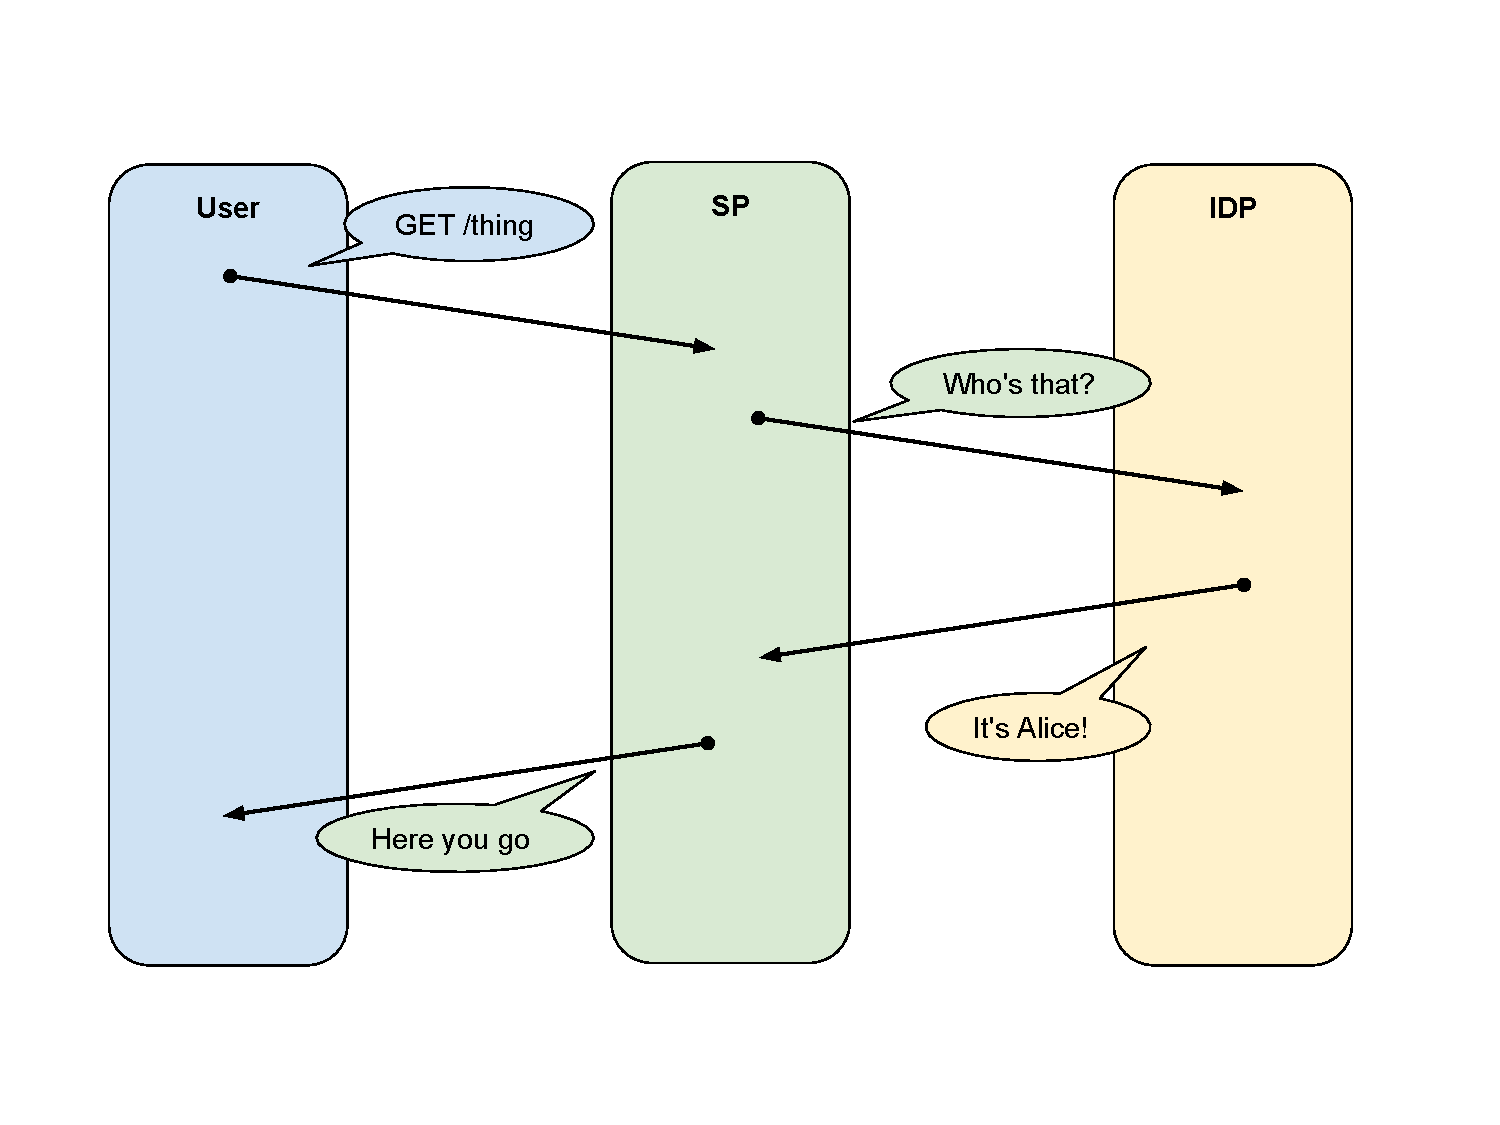
\includegraphics[height=\paperheight]{fedsso-basic.pdf}
\end{frame}

\begin{frame}[plain]
\centering
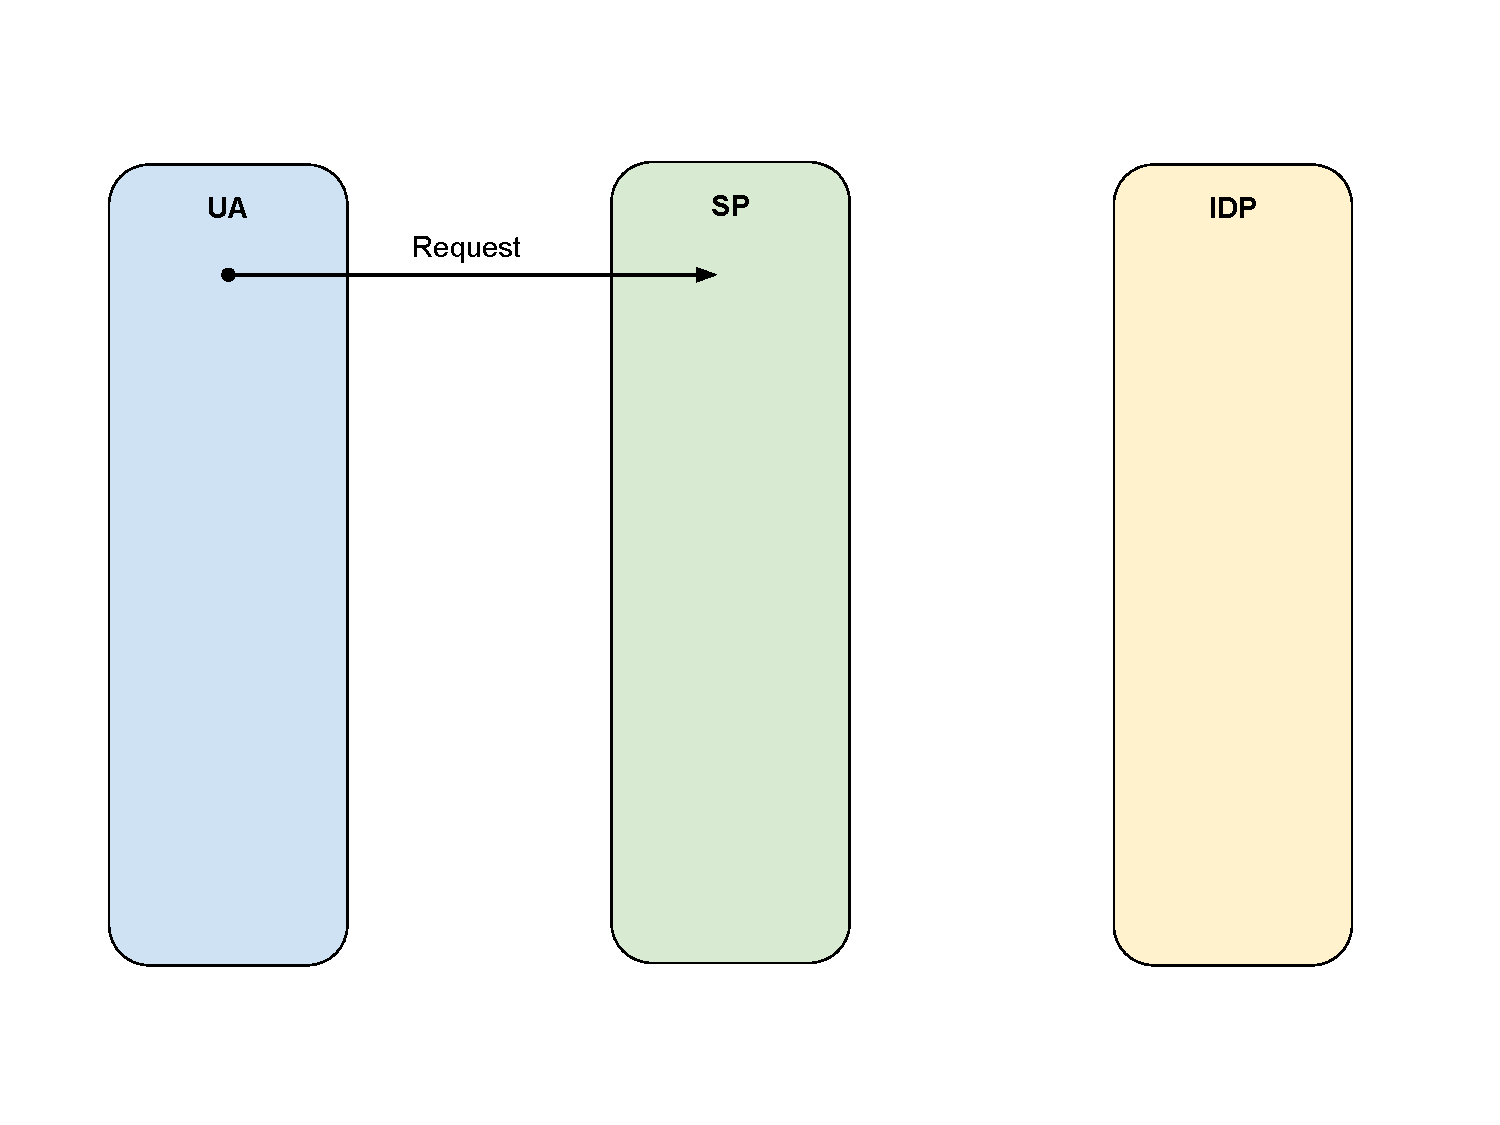
\includegraphics[height=\paperheight]{fedsso-proto-1.pdf}
\end{frame}

\begin{frame}[plain]
\centering
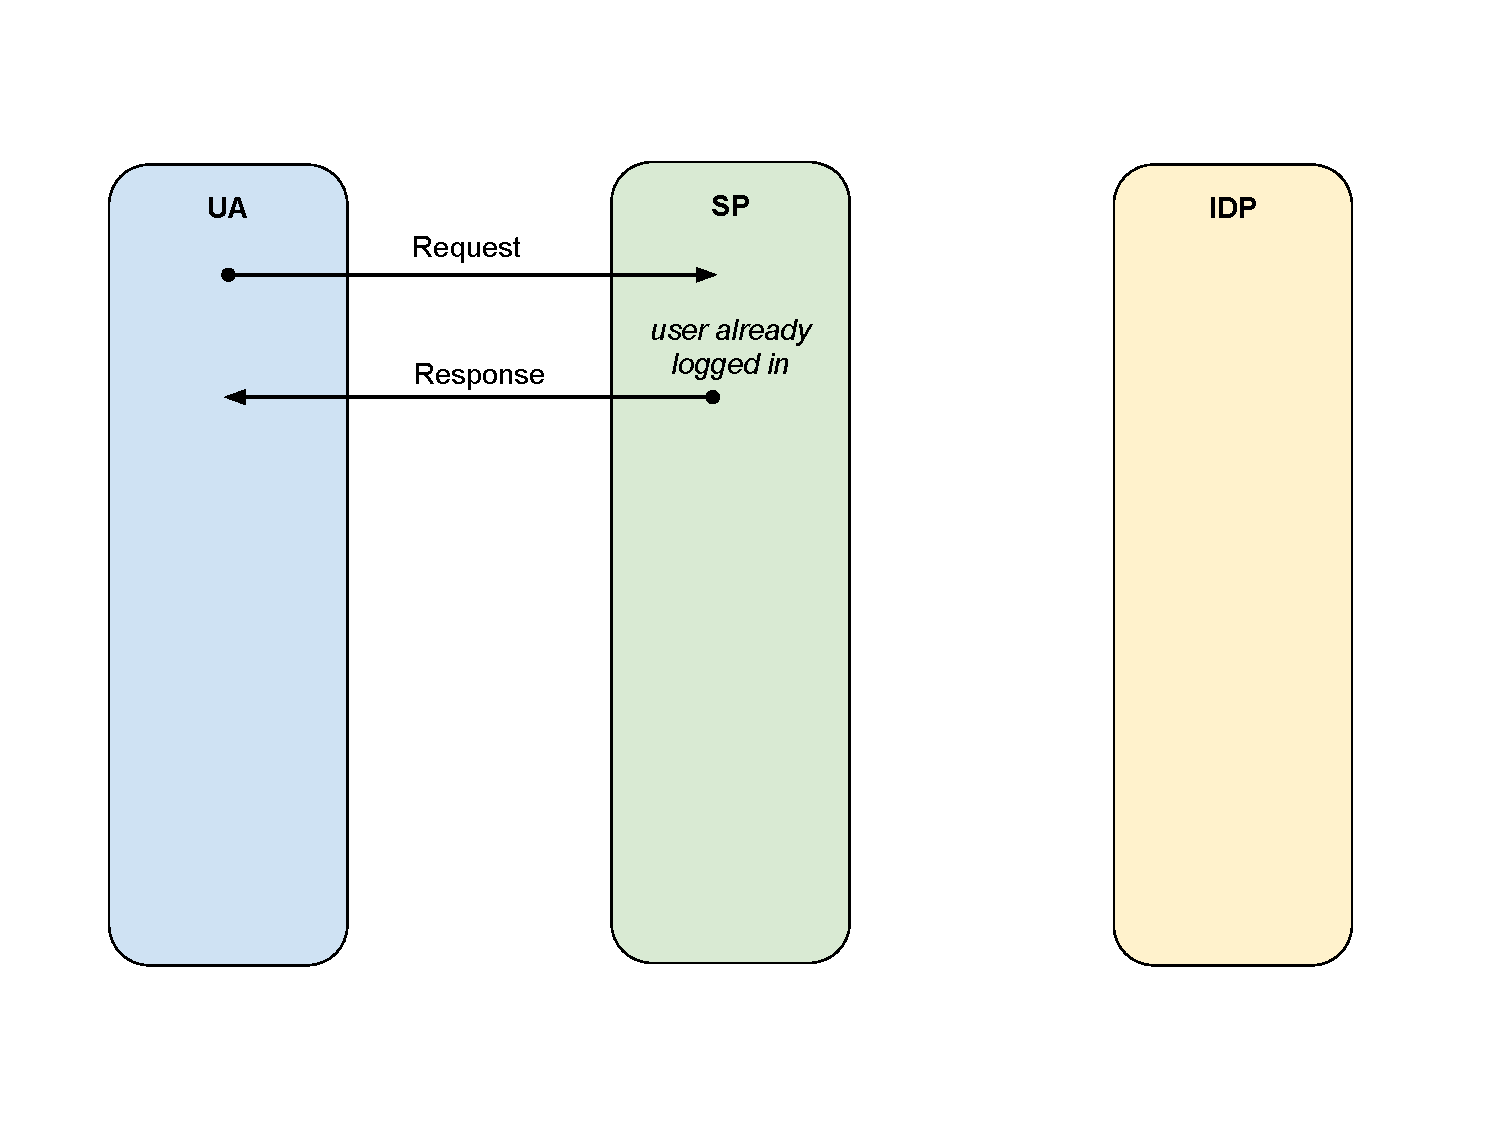
\includegraphics[height=\paperheight]{fedsso-proto-2-logged-in.pdf}
\end{frame}

\begin{frame}[plain]
\centering
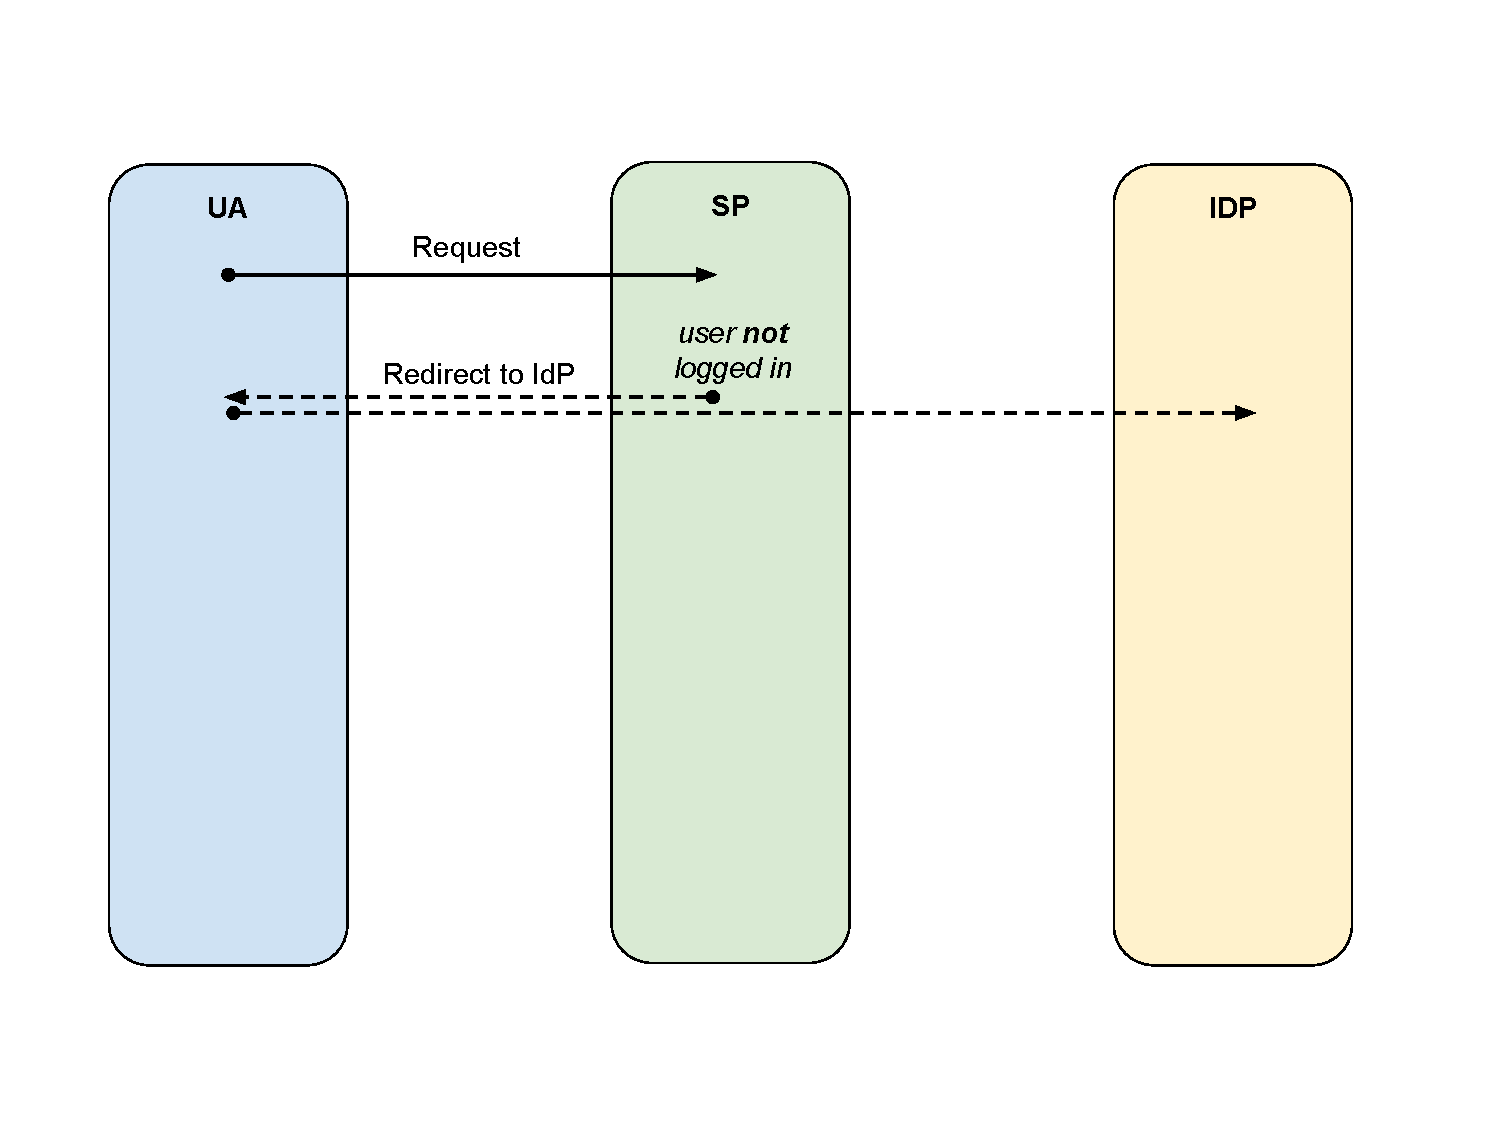
\includegraphics[height=\paperheight]{fedsso-proto-2.pdf}
\end{frame}

\begin{frame}[plain]
\centering
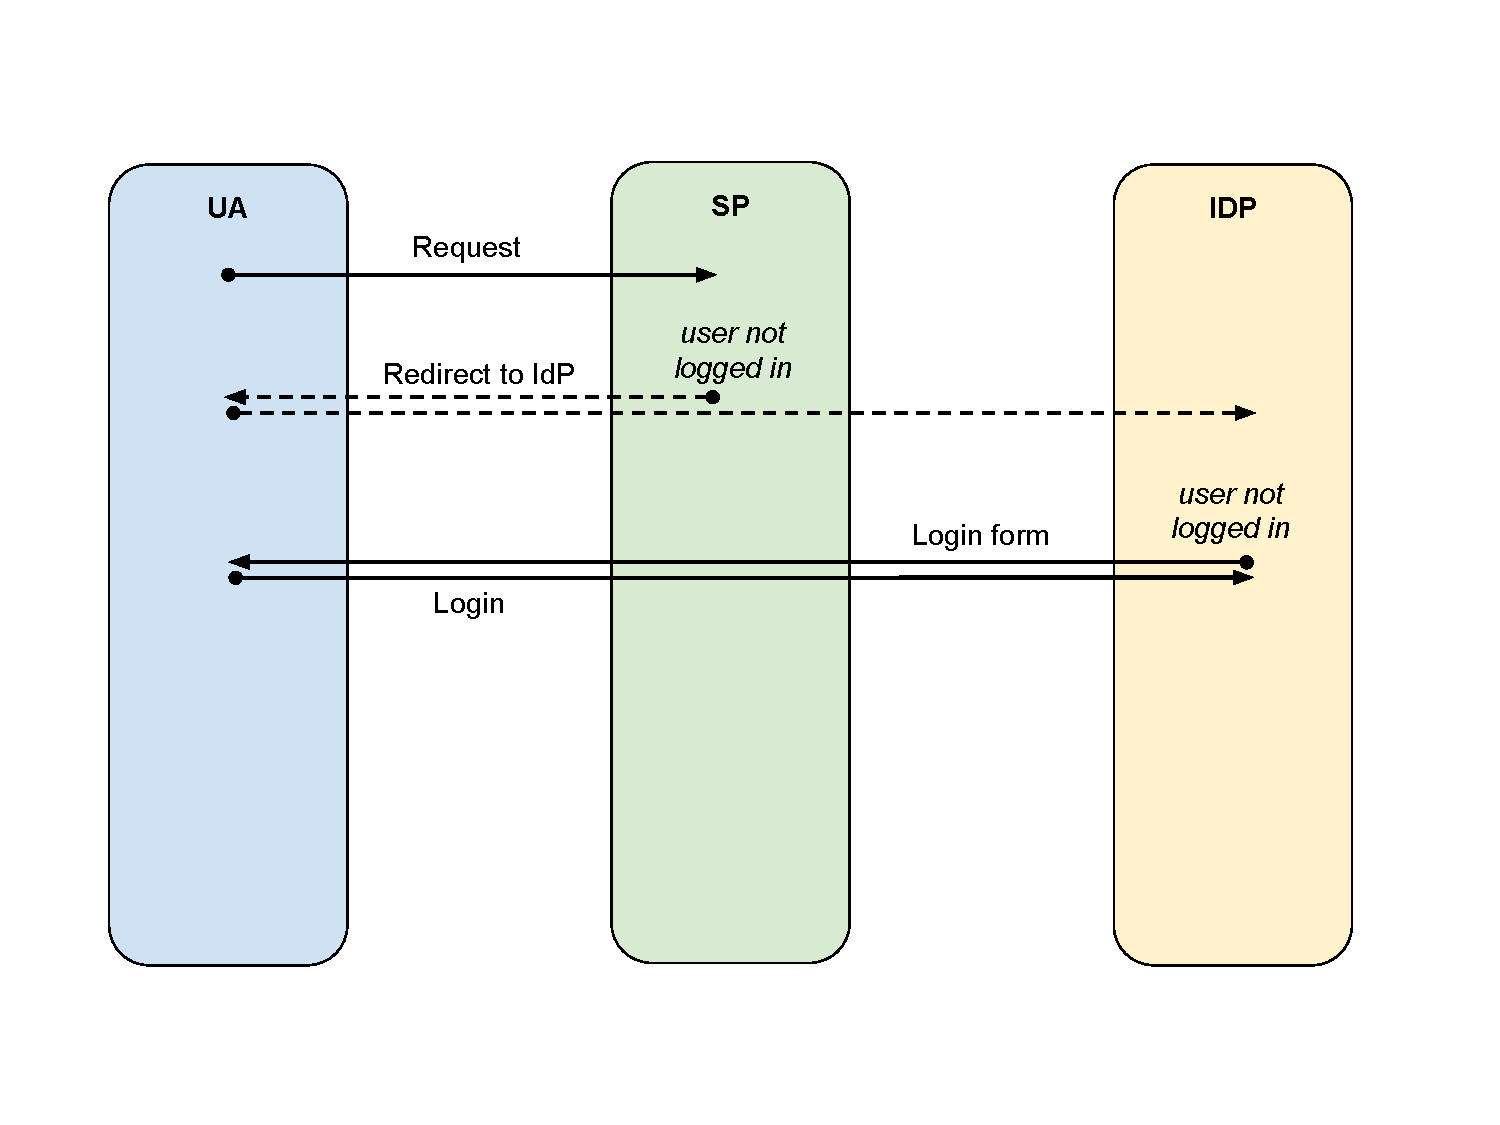
\includegraphics[height=\paperheight]{fedsso-proto-3.pdf}
\end{frame}

\begin{frame}[plain]
\centering
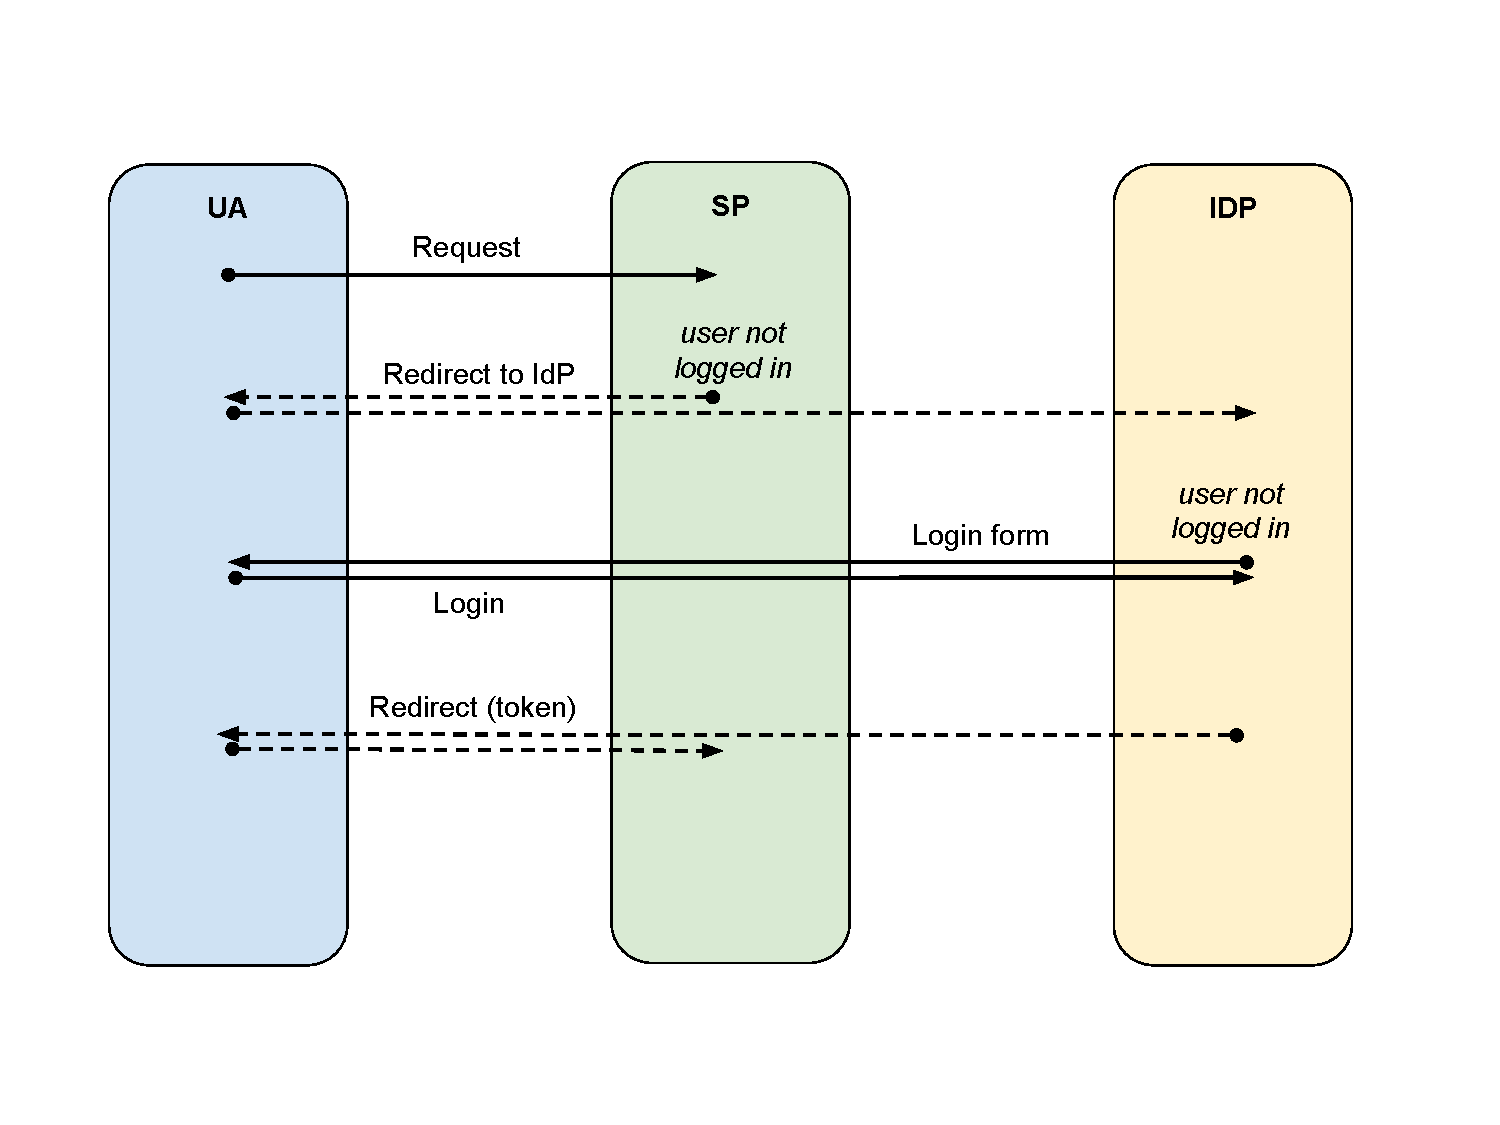
\includegraphics[height=\paperheight]{fedsso-proto-4.pdf}
\end{frame}

\begin{frame}[plain]
\centering
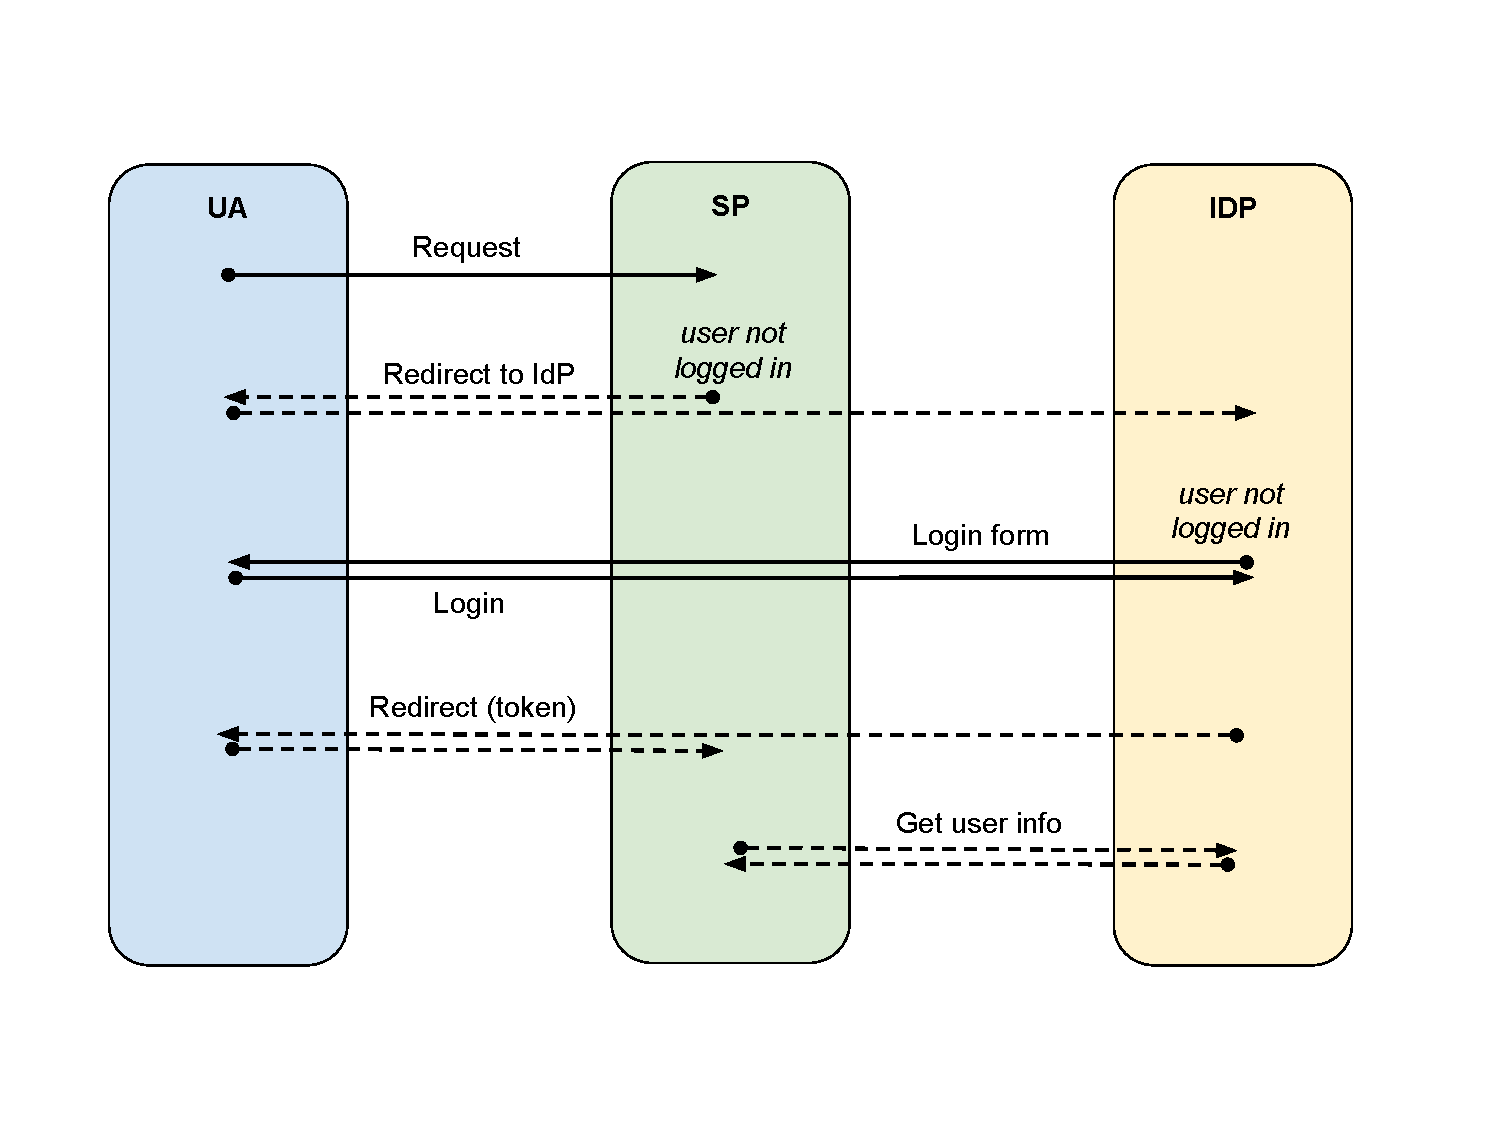
\includegraphics[height=\paperheight]{fedsso-proto-5.pdf}
\end{frame}

\begin{frame}[plain]
\centering
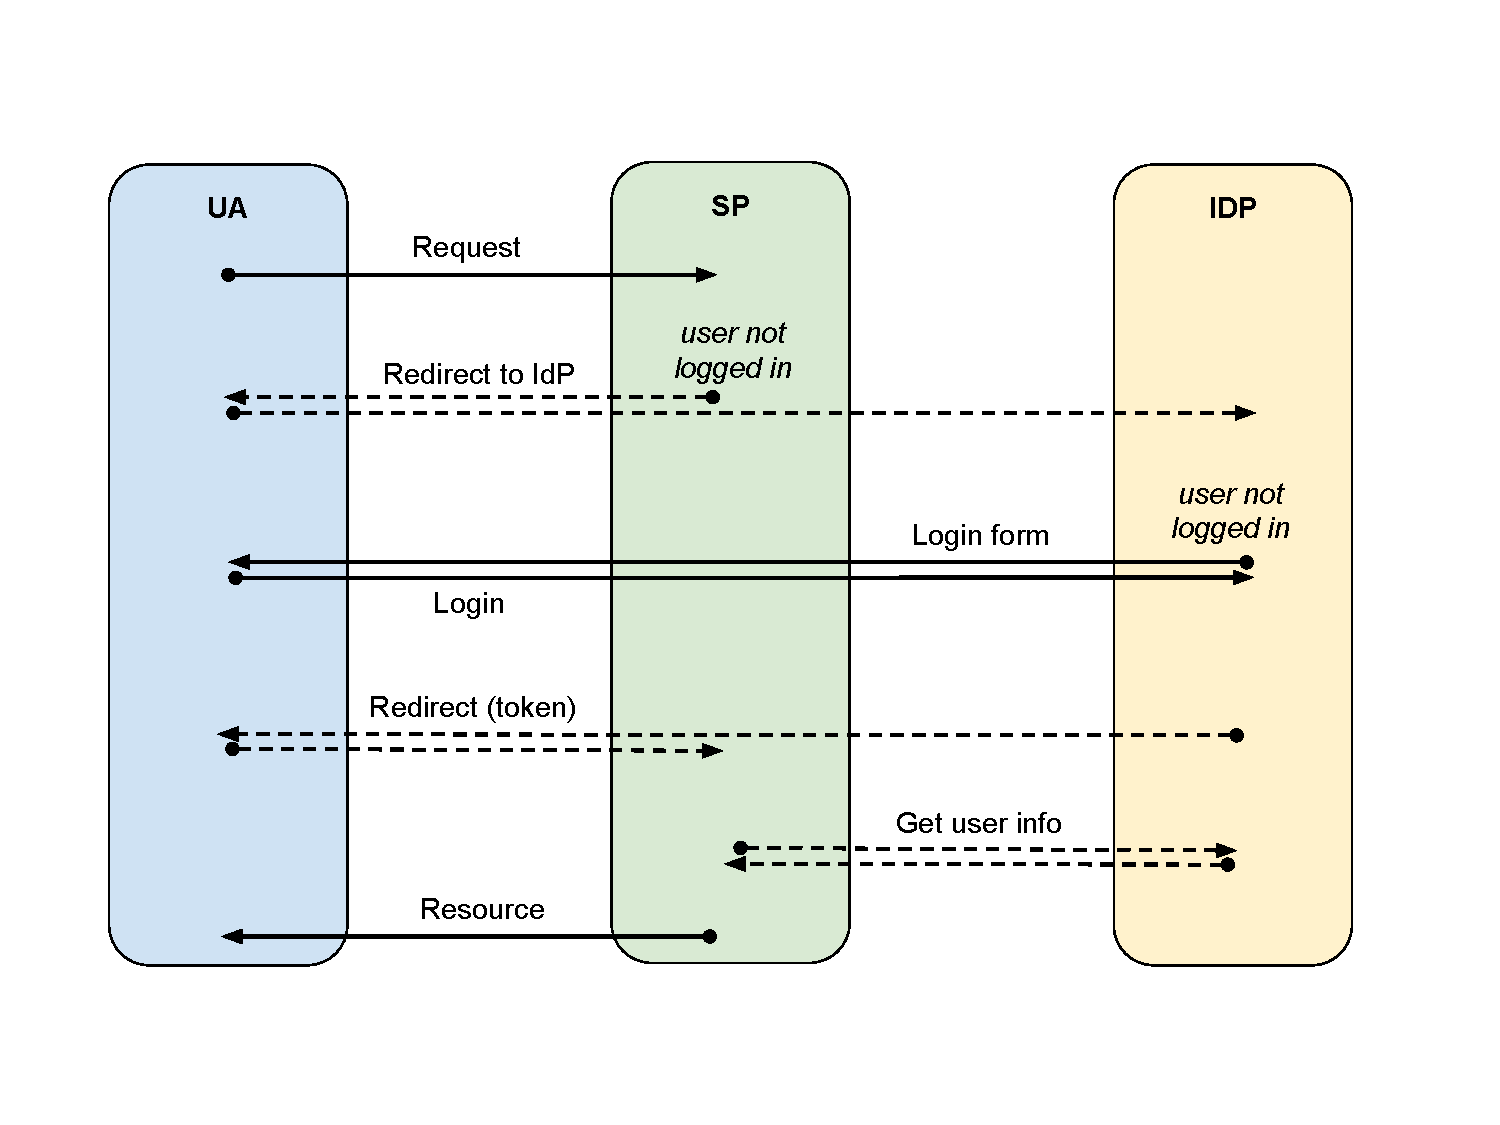
\includegraphics[height=\paperheight]{fedsso-proto-6.pdf}
\end{frame}

\begin{frame}[plain]
\centering
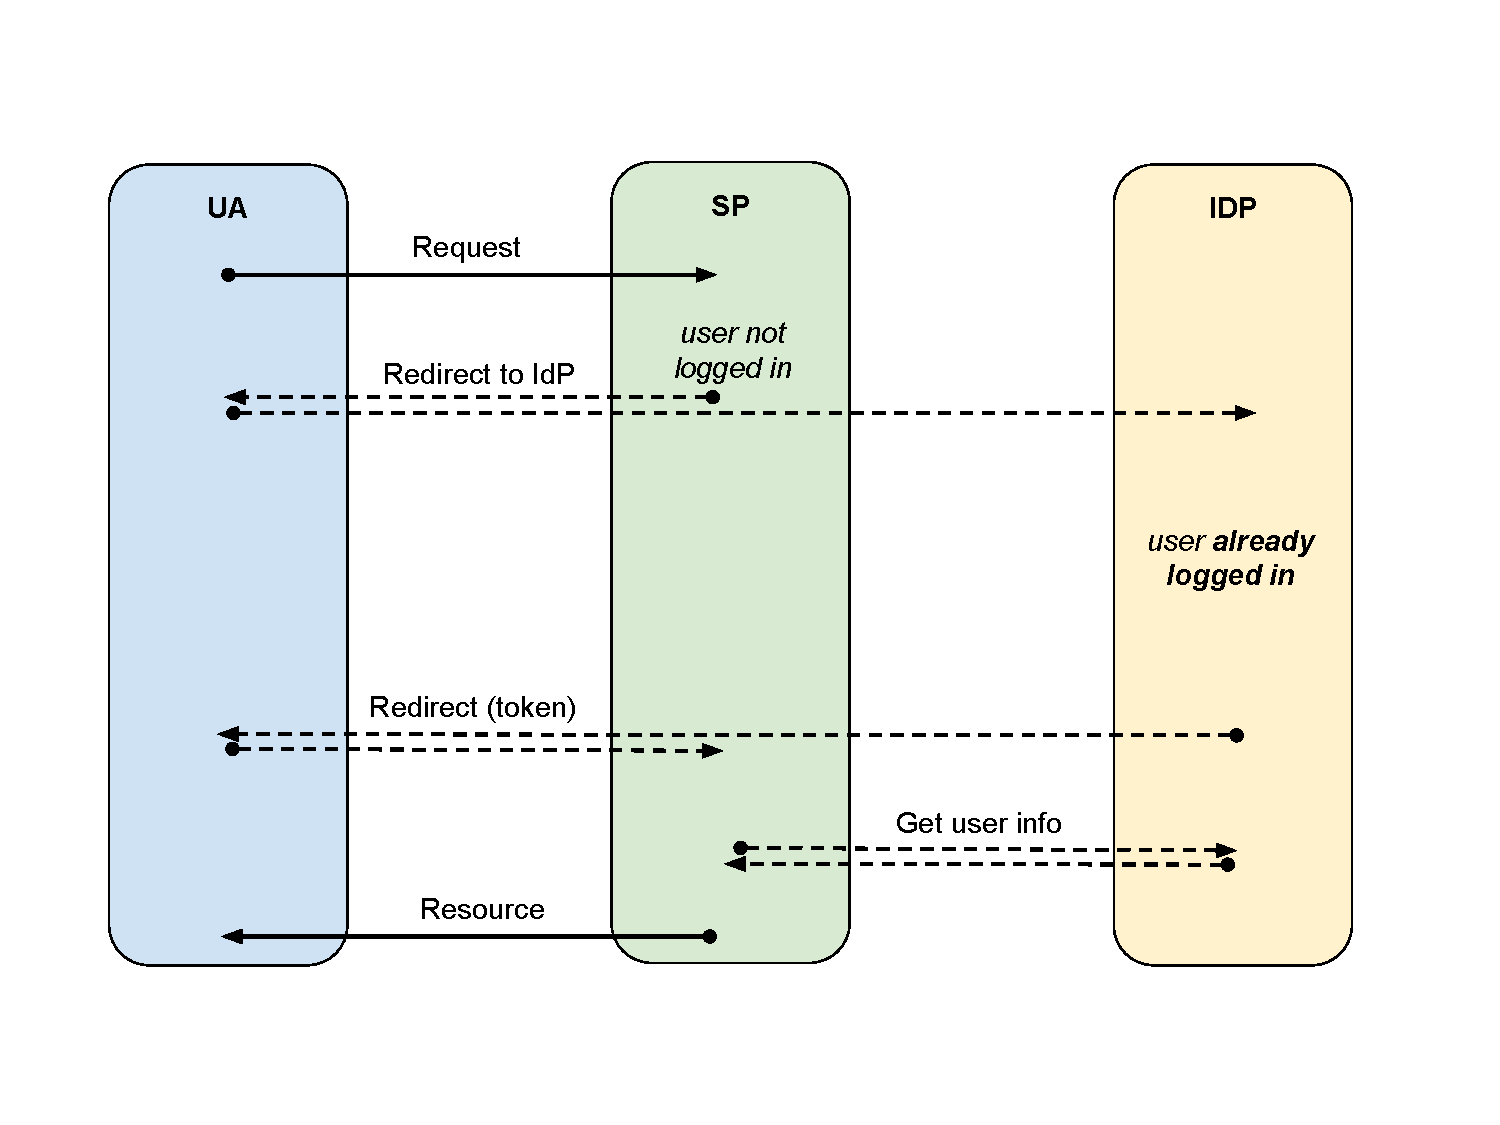
\includegraphics[height=\paperheight]{fedsso-proto-7.pdf}
\end{frame}

\begin{frame}{Protocols - SAML 2.0}

\begin{itemize}
\tightlist
\item \emph{Security Assertion Markup Language}
\item OASIS standard (2005)\footnote{
        \url{http://saml.xml.org/saml-specifications}}
\item XML
\item \emph{single sign-out} capability
\end{itemize}

\end{frame}

\begin{frame}{Protocols - OpenID Connect}

\begin{itemize}
\tightlist
\item OpenID Foundation standard (2014)\footnote{
        \url{https://openid.net/connect/}}
\item based on OAuth 2.0
\item JSON + JWT
\item less client configuration than SAML ({\bf discovery})
\item can support non-browser clients
\end{itemize}

\end{frame}

\begin{frame}{Social login}

\begin{itemize}
\tightlist
\item
  Google, Facebook, Twitter, Linked.in, GitHub, Microsoft, \ldots{}
\item
  typically uses just \textbf{OAuth 2.0}
\item
  integration, account linking
\end{itemize}

\end{frame}

\begin{frame}{Social login - how}

\begin{itemize}
\tightlist
\item
  create an ``app'' with the IDP
\item
  configure SP to request access to user resources
\item
  IDP authenticates user
\item
  user grants access
\item
  IDP redirects back to SP, conveying \emph{token}
\end{itemize}

\end{frame}

\begin{frame}{Enterprise login}

\begin{itemize}
\tightlist
\item
  users already have accounts
\item
  SP requests identity assertions from IDP
\item
  IDP authenticates user (LDAP, Kerberos, \ldots{})
\item
  IDP redirects back to SP, conveying \textbf{assertions}
\end{itemize}

\end{frame}

\begin{frame}{Identity brokers}

\begin{itemize}
\tightlist
\item
  connect SPs with IDPs (many-to-many)
\item
  may support multiple service \emph{realms}
\item
  may support multiple IDP and federation protocols
\end{itemize}

\end{frame}

\begin{frame}[plain]
\centering
\makebox[\textwidth][c]{
    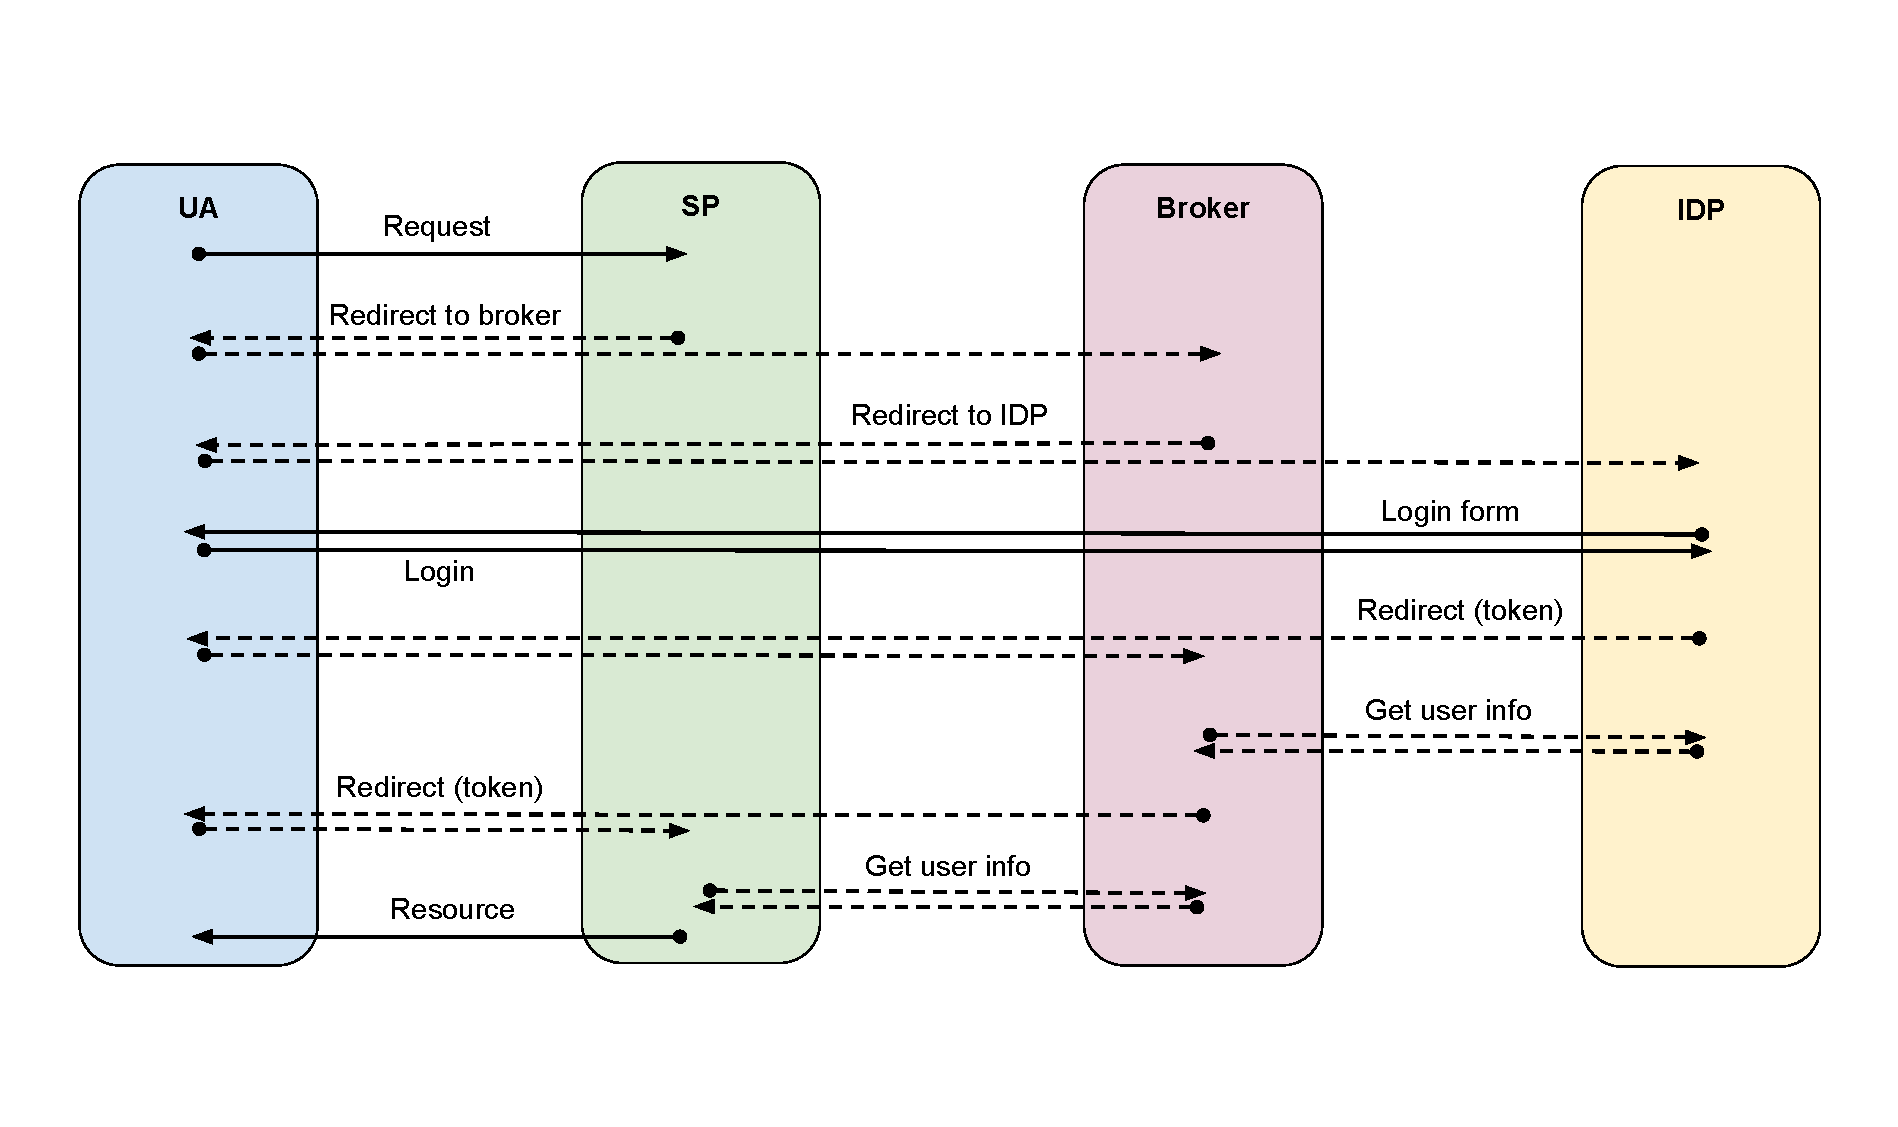
\includegraphics[height=\paperheight]{fedsso-broker.pdf}}
\end{frame}

\begin{frame}{Keycloak}

\begin{itemize}
\tightlist
\item {\bf Open Source} identity broker
\item \url{http://www.keycloak.org/}
\item IDPs: social, SAML, OpenID Connect, LDAP, Kerberos
\item SPs: SAML, OpenID Connect
\item {\em Red Hat Single Sign-On}
\item {\bf Docker} images available\footnote{
        \url{https://hub.docker.com/r/jboss/keycloak/}
    }\textsuperscript{,}\footnote{
        \url{https://github.com/jboss-dockerfiles/keycloak}
    }
\end{itemize}
\end{frame}

\section{Consuming identity assertions}

\begin{frame}[fragile]{SAML SP - \bf \tt
    mod\_auth\_mellon\footnote{\url{https://github.com/UNINETT/mod_auth_mellon}}}

\begin{verbatim}
MellonEnable auth
MellonSPMetadataFile /etc/httpd/saml2/sp-metadata.xml
MellonSPPrivateKeyFile /etc/httpd/saml2/client-private-key.pem
MellonSPCertFile /etc/httpd/saml2/client-cert.pem
MellonIdPMetadataFile /etc/httpd/saml2/idp-metadata.xml

MellonSetEnvNoPrefix REMOTE_USER_EMAIL email

Require valid-user
AuthType Mellon
\end{verbatim}

\end{frame}

\begin{frame}[fragile]{OpenID Connect SP - \bf \tt
    mod\_auth\_openidc\footnote{\url{https://github.com/pingidentity/mod_auth_openidc}}}

\begin{verbatim}
OIDCProviderMetadataURL {IDP_URL}/.well-known/openid-configuration
OIDCRedirectURI http://f26-pyconau.ipa.local/oidc/redirect_uri
OIDCClientID master-oidc
OIDCCryptoPassphrase secret123
OIDCRemoteUserClaim preferred_username

<Location /oidc>
  Require valid-user
  AuthType openid-connect
</Location>
\end{verbatim}

\end{frame}

\begin{frame}[fragile]{NGINX}
\begin{itemize}
\tightlist
\item {\em NGINX Plus} (OpenID Connect; paid)
\item \url{https://github.com/pingidentity/lua-resty-openidc}
\end{itemize}
\end{frame}

\section{Demo}

\section{Python web frameworks}

\begin{frame}{\tt REMOTE\_USER}
\begin{itemize}
\tightlist
\item Standard request variable to identify authenticated user
\item Many apps / frameworks observe it
\item In practice {\tt REMOTE\_USER} is not enough
\end{itemize}
\end{frame}

\begin{frame}{Django - middlewares}
\begin{itemize}
\tightlist

\item {\tt RemoteUserMiddleware}
\item {\tt PersistentRemoteUserMiddleware}
\item {\tt RemoteUserBackend}
%\item {\tt RemoteUserAttrMiddleware} reads attributes and updates user object

\end{itemize}
\end{frame}

\begin{frame}[fragile]{Django - configuration}
\begin{Shaded}
\begin{Highlighting}[]
\NormalTok{MIDDLEWARE_CLASSES }\OperatorTok{=} \NormalTok{(}
 \NormalTok{...}
 \StringTok{'django.contrib.auth.middleware.AuthenticationMiddleware'}\NormalTok{,}
 \StringTok{'django.contrib.auth.middleware.PersistentRemoteUserMiddleware'}\NormalTok{,}
 \StringTok{'identity.external.RemoteUserAttrMiddleware'}\NormalTok{,}
 \NormalTok{...}
\NormalTok{)}

\NormalTok{AUTHENTICATION_BACKENDS }\OperatorTok{=} \NormalTok{(}
  \StringTok{'django.contrib.auth.backends.RemoteUserBackend'}\NormalTok{,}
  \StringTok{'django.contrib.auth.backends.ModelBackend'}\NormalTok{,}
\NormalTok{)}
\end{Highlighting}
\end{Shaded}
\end{frame}

\begin{frame}{Django - login form}
\begin{itemize}
\tightlist

\item {\tt login} view does not observe {\tt REMOTE\_USER}

\item workaround: wrap {\tt django.contrib.auth.views.login}

    \begin{itemize}
    \tightlist
    \item redirect if {\tt request.user.is\_authenticated()}
    \item update {\tt urls.py} to use wrapped view
    \end{itemize}

\end{itemize}
\end{frame}

\begin{frame}{Django - resources}
\begin{itemize}
\tightlist

\item \url{https://docs.djangoproject.com/en/1.11/howto/auth-remote-user/}
\item \url{http://www.adelton.com/django/external-authentication-for-django-projects}
\item \url{https://djangopackages.org/grids/g/oidc/}
\item \url{https://djangopackages.org/packages/p/djangosaml2/}
\item \url{https://djangopackages.org/packages/p/python-social-auth/}

\end{itemize}
\end{frame}

\begin{frame}{General guidelines}
\begin{itemize}
\tightlist
\item use {\bf middleware(s)} to interpret request environment
\item map remote {\bf roles} to app roles
\item users: transient or persisted?
\item {\bf tweak login view} as needed
\end{itemize}
\end{frame}

\section{Wrapping up}

\begin{frame}{Security}
\begin{itemize}
\tightlist
\item use {\bf TLS} everywhere
\item how secure are the {\bf libraries}?
\item how secure are the {\bf
    protocols}?\footnote{
        \href{https://arxiv.org/pdf/1601.01229v2.pdf}{
            A Comprehensive Formal Security Analysis of OAuth 2.0
        }
    }\textsuperscript{,}\footnote{
        \href{https://arxiv.org/pdf/1704.08539.pdf}{
            The Web SSO Standard {\em OpenID Connect}:
            In-Depth Formal Security Analysis and Security Guidelines
        }
    }\textsuperscript{,}\footnote{
        \href{https://ai-lab.it/armando/pub/fmse9-armando.pdf}{
            Formal Analysis of SAML 2.0 Web Browser Single Sign-On:
            Breaking the SAML-based Single Sign-On for Google Apps
        }
    }
\item preventing token / data interception at UA
\end{itemize}
% guidelines:
% - include issues in authz endpoint response
% - fresh state nonce for each login attempt
% - use referrer policies to prevent code/token/state leakage
%   (header 'Referrer-Policy: ...')
% - all the usual stuff: TLS, SRI, secure, HttpOnly cookies,
%   replace session cookie upon login (avert session fixation
%   attack), etc.
\end{frame}

\begin{frame}[plain]
\centering
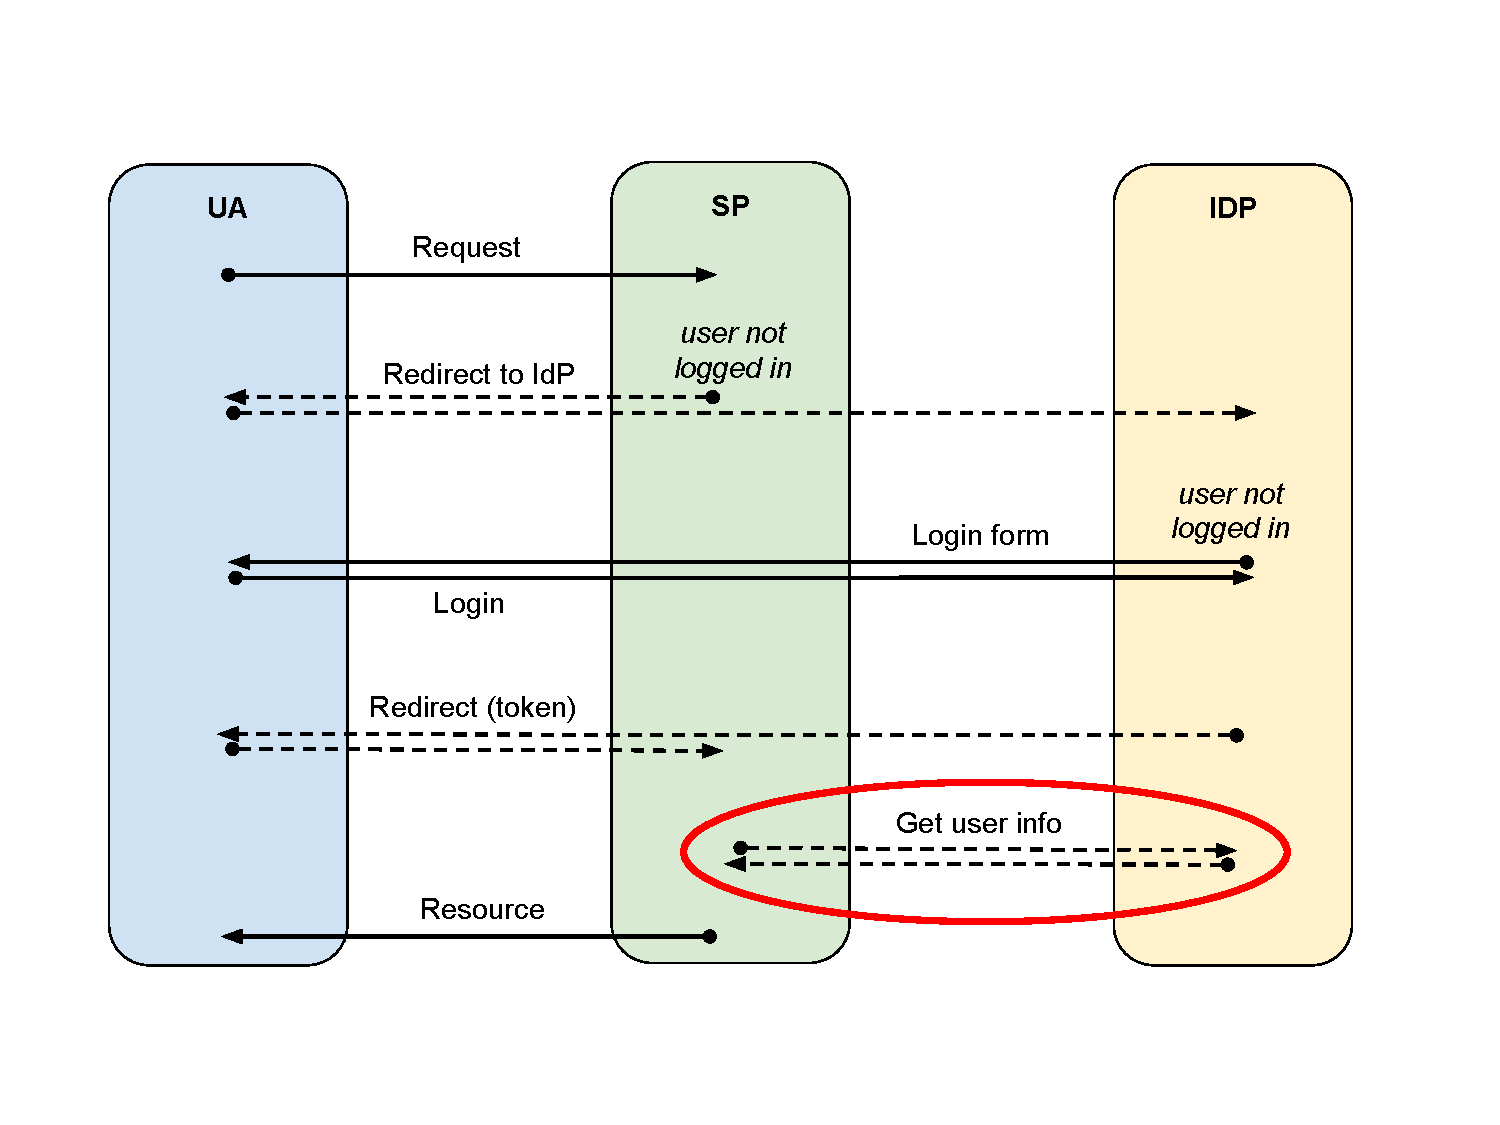
\includegraphics[height=\paperheight]{fedsso-proto-6-getuserinfo.pdf}
\end{frame}

\begin{frame}{Challenges}

\begin{itemize}
\tightlist
\item testing
\item email verification
\item account linking\footnote{
        \url{https://stackoverflow.com/questions/6666267/architecture-for-merging-multiple-user-accounts-together}
    }\textsuperscript{,}\footnote{
        \url{https://www.sitepoint.com/social-network-authentication-merging-accounts/}
    }
\end{itemize}
% notes:
%   - separate models for each IDP, and for the app.  "link" them
%   - offer "link/connect account" option for logged-in users
%   - offer (but DO NOT REQUIRE) to merge accounts if new social
%     login has email matching existing account
%   - post-facto account linking - what to do with content?
%     that's up to you!
%   - requirement: do not make your primary key the social username
\end{frame}

\begin{frame}{SAML or OpenID Connect?}
\begin{itemize}
\tightlist
\item if you're implementing new services: OpenID Connect
\item if it's a {\bf mobile} app: OpenID Connect
\item if the SP only speaks one or the other: use that
\item if you have SAML {\em and} OpenID Connect SPs: {\bf broker}
\end{itemize}
\end{frame}

\begin{frame}{Single sign-out}
\begin{itemize}
\tightlist
\item what happens when user signs out of IDP?
\item supported by SAML; {\em draft spec} for OpenID Connect
\end{itemize}
\end{frame}

\begin{frame}[plain]
\centering
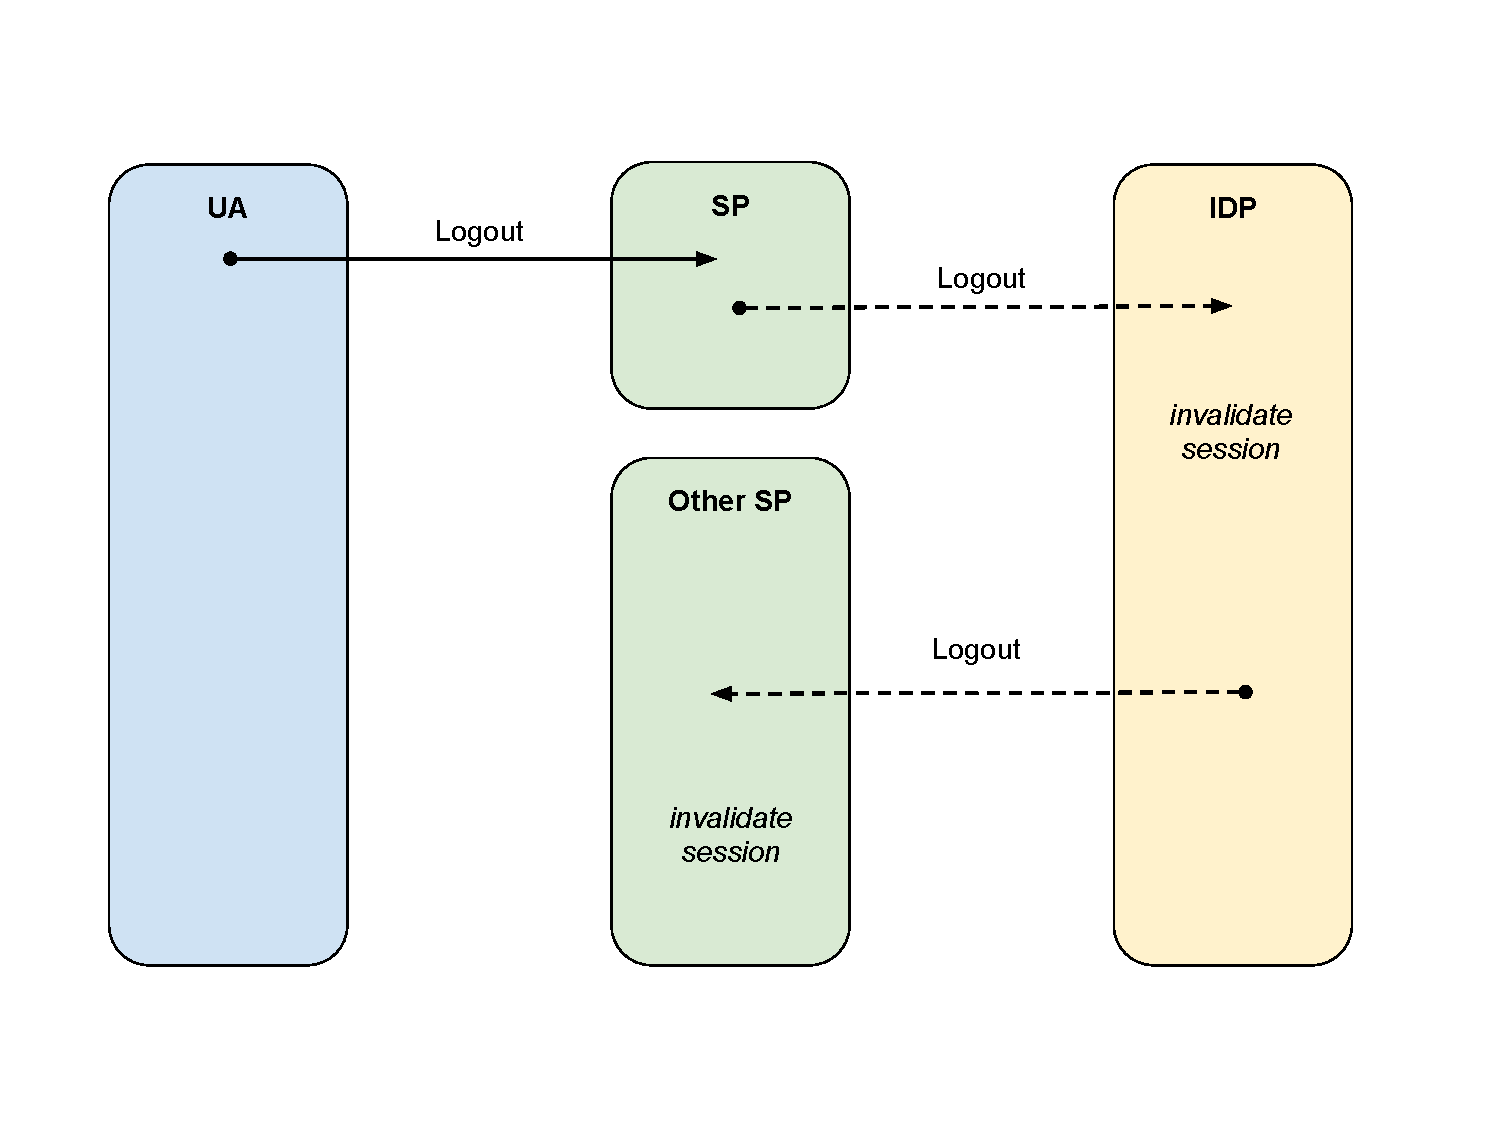
\includegraphics[height=\paperheight]{fedsso-logout-backchannel.pdf}
\end{frame}

\begin{frame}[plain]
\centering
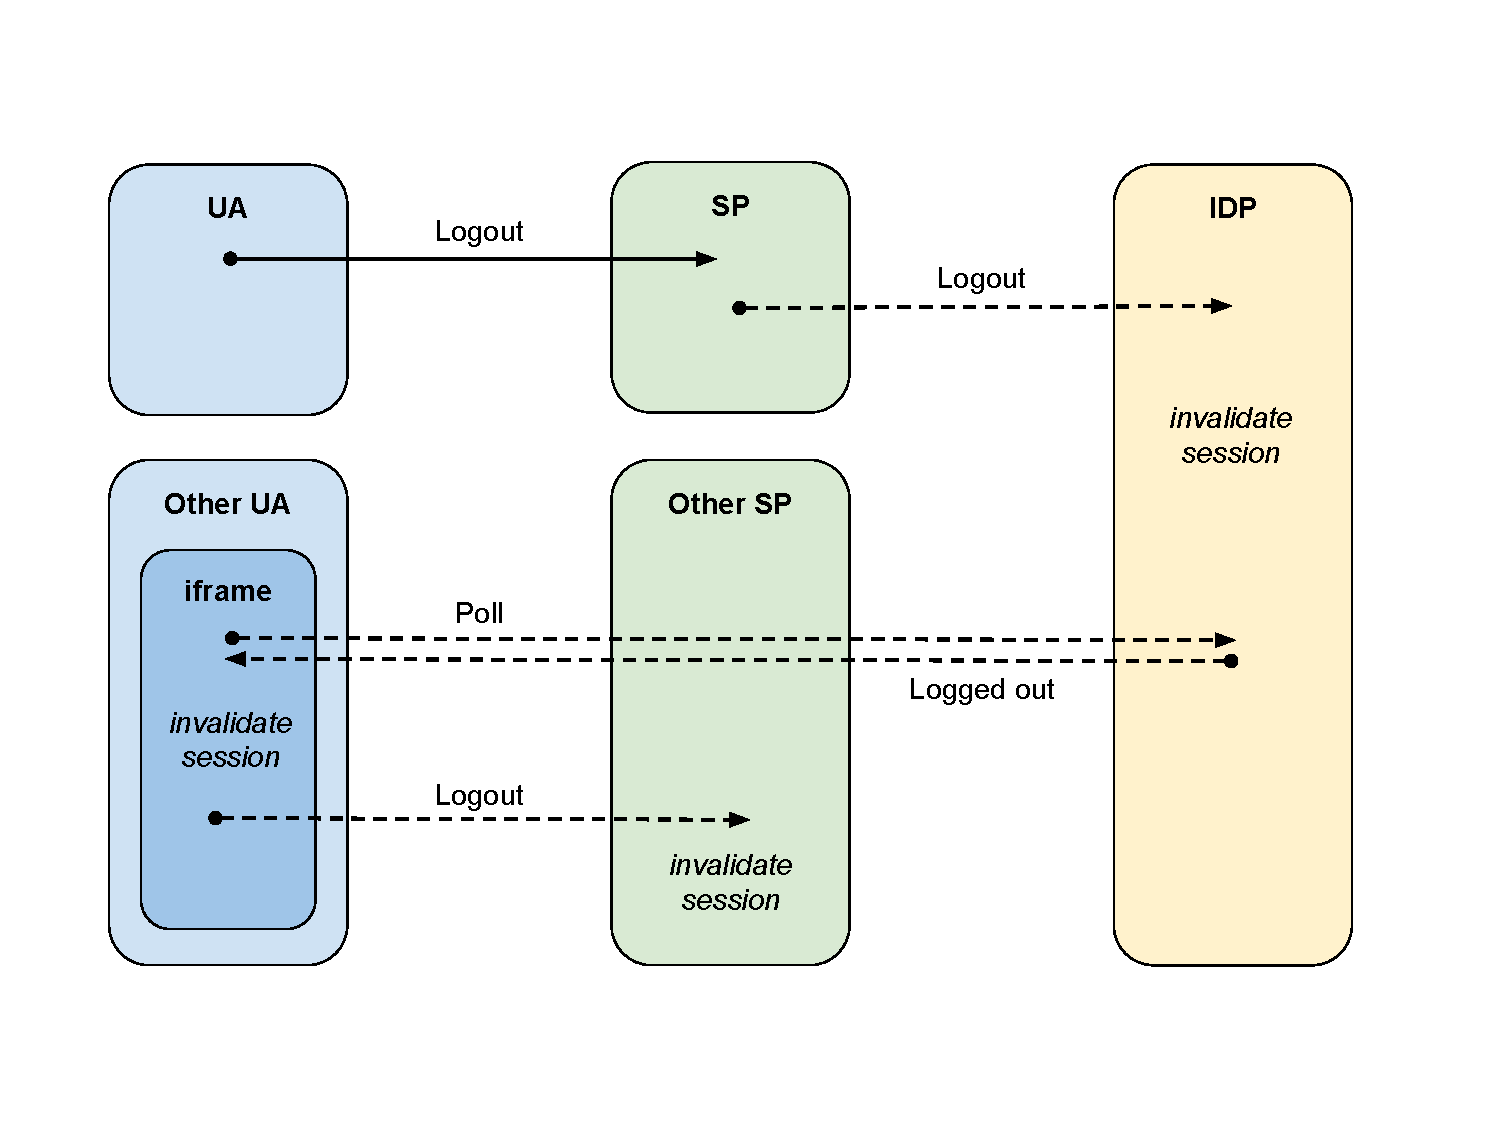
\includegraphics[height=\paperheight]{fedsso-logout-frontchannel.pdf}
\end{frame}

\begin{frame}{Recap}

\begin{itemize}
\tightlist
\item {\bf Socialise} or {\bf centralise} your authentication
\item \textbf{Identity brokers} can do a lot of the heavy lifting
\item \textbf{Web servers} can present a consistent view to apps
\end{itemize}

\end{frame}

\begin{frame}[plain]

%\begin{columns}

  %\begin{column}{.4\textwidth}
  %  put something here? % \includegraphics[width=1.2\textwidth]{FILENAME}
  %\end{column}

  %\begin{column}{.6\textwidth}

    \setlength{\parskip}{.5em}

    { \centering

    \input{cc-by-ARTIFACT.pdf_tex}
    \\
    { \scriptsize
    Except where otherwise noted this work is licensed under
    }\\
    { \footnotesize
    \textbf{http://creativecommons.org/licenses/by/4.0/}
    }

    \bigskip
    \Large

    \url{https://speakerdeck.com/frasertweedale}

    \texttt{@hackuador}

    }
  %\end{column}

%\end{columns}

\end{frame}

\end{document}
